\documentclass[table, 12pt]{article}
\usepackage{graphicx}
\usepackage[T1]{fontenc}
\usepackage{tocloft}
\usepackage{todonotes}
\usepackage{caption}
\usepackage{hyperref}
\usepackage{booktabs}
\usepackage{listings}
\usepackage{pdfpages}
\usepackage{pdflscape}
\usepackage{textpos}
\usepackage{scrhack}
\usepackage{xcolor}
\usepackage{float}
\usepackage{longtable}
\usepackage{enumitem}
\usepackage{tasks}
\usepackage{tabularx}
\usepackage{titlesec}
\usepackage{listing}
\usepackage{graphicx}


\titleformat{\paragraph}
{\normalfont\normalsize\bfseries}{\theparagraph}{1em}{}
\titlespacing*{\paragraph}
{0pt}{3.25ex plus 1ex minus .2ex}{1.5ex plus .2ex}

\begin{document}
\begin{titlepage}
    \centering
    {\scshape\large AY 2020/2021 \par}
    \vfill
    
\includegraphics[width=100pt]{assets/logo-polimi-new}\par\vspace{1cm}
    {\scshape\LARGE Politecnico di Milano \par}
    \vspace{1.5cm}
    {\huge\bfseries Middleware Technologies\\Distributed Node-Red Flows\par}
    \vspace{2cm}
    {\Large {Federico Armellini\quad Luca Pirovano\quad Nicolò Sonnino}\par}
    \vfill
    {\large Professor\par
        Luca \textsc{Mottola}}
    \vfill
    {\large \textbf{Version 1.0}\\ \today \par}
\end{titlepage}
\hypersetup{%
    pdfborder = {0 0 0}
}
\thispagestyle{plain}
\pagenumbering{gobble}
\mbox{}
\newpage
\pagenumbering{roman}
\tableofcontents
\newpage
\pagenumbering{arabic}
\section{Introduction}
\subsection{Description of the project}
You are to implement an architecture that allows Node-red flows to span multiple devices. Normally, a
Node-red flow executes locally to the machine where it is installed. Instead, consider multiple Node-red
installations that 
\begin{enumerate}
    \item register to a central repository that maintains information on all running installations
    \item can exchange messages among them by logically connecting the output of a node in one installation to the input
    of another node in a different installation.
\end{enumerate}
Addressing of Node-red installations must be content-based, that is,
the target Node-red installations that receive the messages cannot be determined based on their IP address or
some other form of machine-level identifier. You need to demonstrate that a flow developed to be executed on a
single Node-red installation may be split across two or multiple Node-red machines with a limited set of
modifications to the flow itself.

\section{Solution Overview}
\subsection{General Architecture}
\begin{figure}
    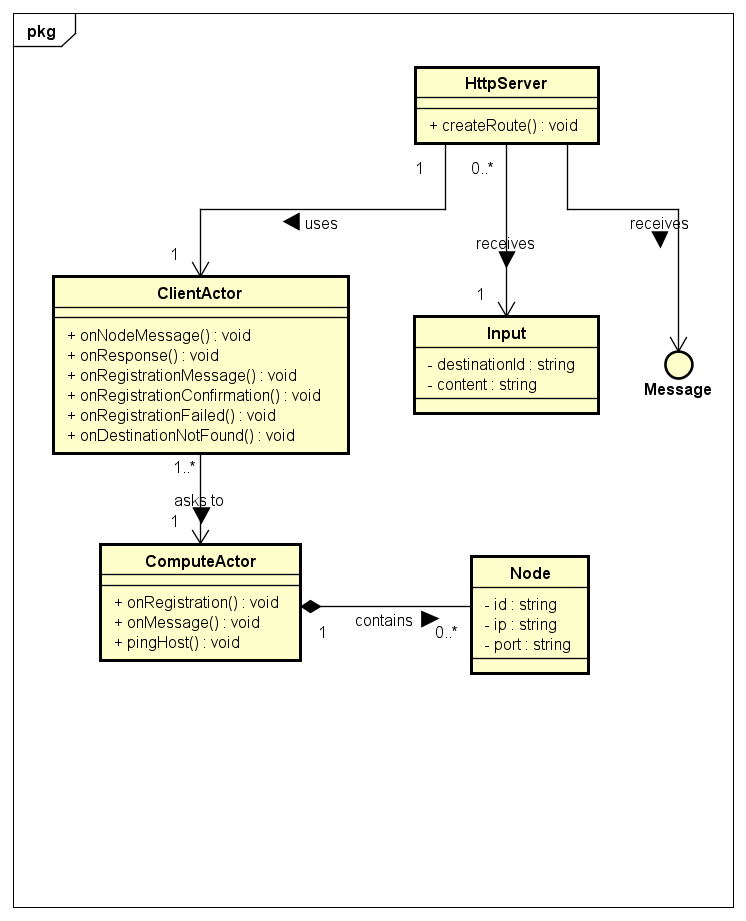
\includegraphics[width=\textwidth]{assets/UML.png}
    \caption{UML Class Diagram of the proposed solution}
    \label{uml}
\end{figure}
Our solution mixes the Node-Red technology for front-end nodes with the Apache Akka technology for backend and syncronization of the different instances.

As shown in figure \ref{uml}, the application coordination backend will be divided in several components:
\begin{itemize}
    \item \textbf{HttpServer:} it is the exposed interface, which duty is to collect requests coming from the different Node-Red instances and perform the requested actions. It is implemented through the Akka Http Suite;
    \item \textbf{ClientActor:} it is the Akka actor on the http server side, which has to collect the actions to be performed from the http server and send them to the compute actor, which will return a result;
    \item \textbf{ComputeActor:} it is the model part of our system, which contains the application logic. In fact, it receives requests from the ClientActor, performs the requested action and returns a result to be sent to the Node-Red instance in question.
    \item \textbf{Input and Node:} they are a representation in our model of the input collected by the http server and the node which is stored in a list with the other ones at the compute actor side. They are parsed automatically from json input through the Jackson Java Library.
    \item \textbf{Message:} it is an interface representing a message which can travel from the client actor to the compute one.
\end{itemize}

\subsection{Flow of an execution}
Everything starts from the Node-Red instance. In fact, a node needs to register contacting the server API (\textit{http://<server\_url>:<port>/register}) with an HTTP POST request.
The node must pass its identifier, its ip address and the port which Node-Red instance is running on.

Once registered, the node can call the API for passing a message to another one (\textit{http://<server\_url>:<port>/send}) with an HTTP POST request. In this case, it must pass the destination id and the content of the message.

All messages must be sent using the JSON standard for message formatting.

When the HTTP server receives a \textit{register} or \textit{send} message, it triggers the client actor which contacts the compute one:
\begin{itemize}
    \item in case of register, the compute actor checks if the node is not in the list of already existent ones; in that case, it simply adds it, otherwise it returns an exception to the client;
    \item in case of send, the compute actor checks if the destination exists and, in that case, returns the information about the destination, so that http server can send the message to it.
\end{itemize}

When the Client Actor receives a response from the Compute one, it returns a representation to the HTTP server. In case of register procedure, http server simply returns a status code; in the send one, instead, if the destination was found the http server opens a websocket and send the message to the correct node.

\subsubsection{Disconnection}
In case a node loses the connection with the backend, it is unregistered at the successive send operation. 
In fact, when a message must be sent to a client, a ping is performed to check if the destination node is still alive.

When a client is not reachable, it is immediately removed from the nodes list.

\subsection{Assumptions}
\begin{enumerate}[label=\textbf{A\arabic*:}]
    \item The set of the running Node-Red installation is dynamic, which means that they can join or leave at any moment.
    \item The solution is agnostic to the content of the message.
    \item On a send message, if the destination node is not specified, the destination is chosen randomly. Of course we must assume that, in this case, all the receiving node-red installation can handle this request.
\end{enumerate}


\end{document}